% !TEX encoding = UTF-8 Unicode

\documentclass[aspectratio=169]{beamer}
\usepackage[utf8]{inputenc}

%% BIB
\usepackage[
  style=authoryear,
  backend=biber,
  url=false,
  maxcitenames=2,
  uniquename=false,
  uniquelist=false
]{biblatex}
%\addbibresource{?.bib}

%% GRAPHICS

\usepackage{graphicx}
\graphicspath{{images/},{figures/}}
\usepackage{tikz}

%% COLORS
\definecolor{UWRed}{HTML}{C5050C}
%\definecolor{StrongBlue}{HTML}{3F8FD2}
%\definecolor{StrongGreen}{HTML}{36C88E}
%\definecolor{StrongRed}{HTML}{9B0000}
%\definecolor{MyC}{HTML}{009999}
%\definecolor{MyM}{HTML}{990099}
%\definecolor{MyY}{HTML}{999900}
%\definecolor{MyR}{HTML}{990000}
%\definecolor{MyG}{HTML}{009900}
%\definecolor{MyB}{HTML}{000099}
%\definecolor{ActionRed}{HTML}{990000}

%% SLIDE COLOR SETTINGS
\setbeamercolor{structure}{fg=UWRed}
\setbeamercolor{title page}{fg=white}
\setbeamercolor{title}{fg=white}

%% RM NAV SYMBOLS
\setbeamertemplate{navigation symbols}{}

%% FONTS
\setbeamerfont{title}{size=\huge\bfseries}

%% DRAWING
%\usetikzlibrary{}

\def\firstcircle{(90:0.3cm) circle (0.6cm)}
\def\secondcircle{(210:0.3cm) circle (0.6cm)}
\def\thirdcircle{(330:0.3cm) circle (0.6cm)}

%% LOGO on slides
\logo{\begin{tikzpicture}[overlay]
  \node[anchor=north east,inner sep=0] at (0,86mm) {
\includegraphics[height=10mm]{SMPH_color-flush.pdf}};
\end{tikzpicture}}

%% CONTENT BEGINS

\title{Anchors (and other) High-Precision Model-Agnostic Explanations}
\subtitle{AIRG Presentation}
\author{Yuriy Sverchkov}
\institute{University of Wisconsin--Madison}
\date{October 31, 2018}

\begin{document}

  {
    \setbeamertemplate{background canvas}{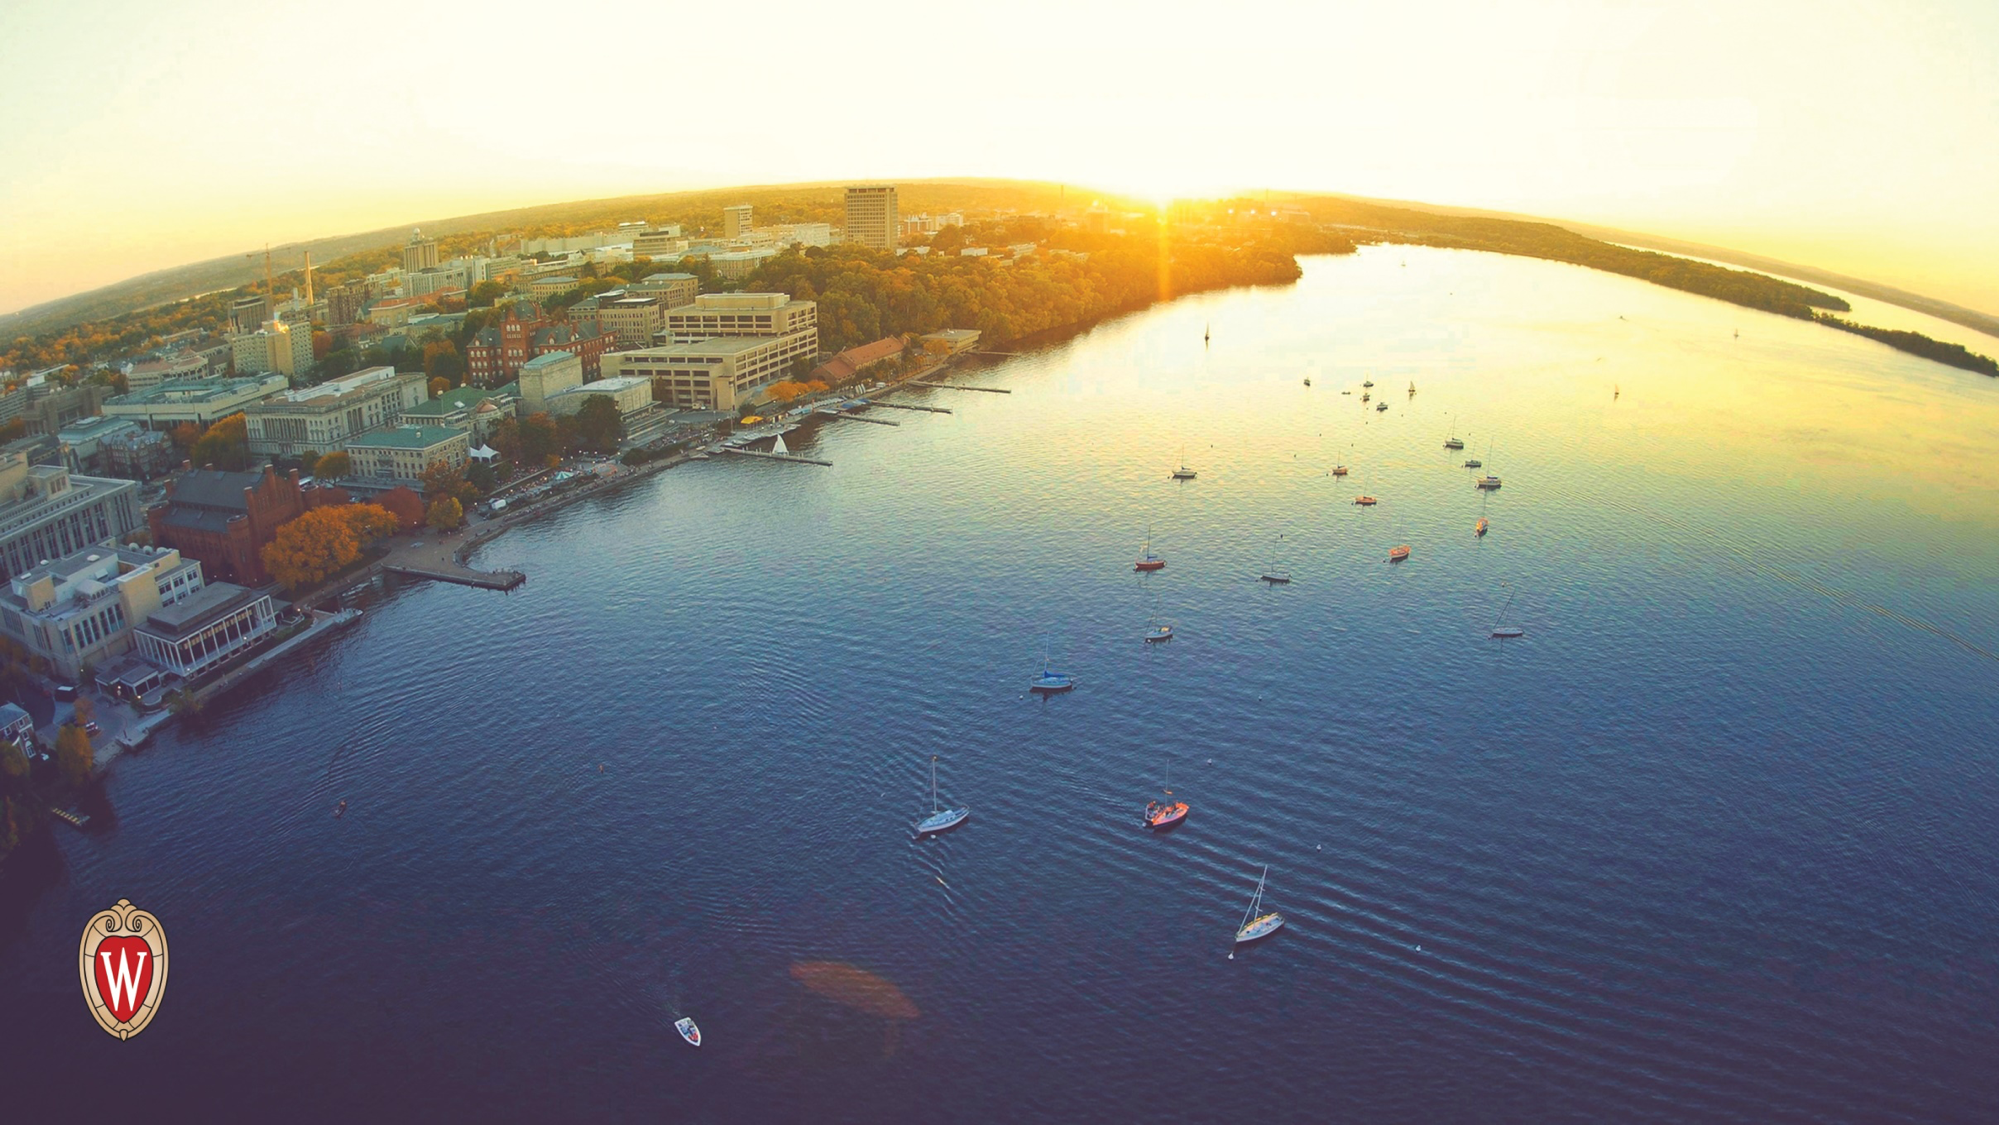
\includegraphics[width=\paperwidth]{UW-lake.png}}
    \begin{frame}[plain]
      \vskip4cm
      \titlepage
    \end{frame}
  }

\begin{frame}{First, some context}
Why are we explaining things?
\end{frame}
  
%%% FRAMEBREAK %%%

\begin{frame}{Prior work}
\begin{itemize}
	\item TERPAN
	\item LIME
	\item that thingie for images
\end{itemize}
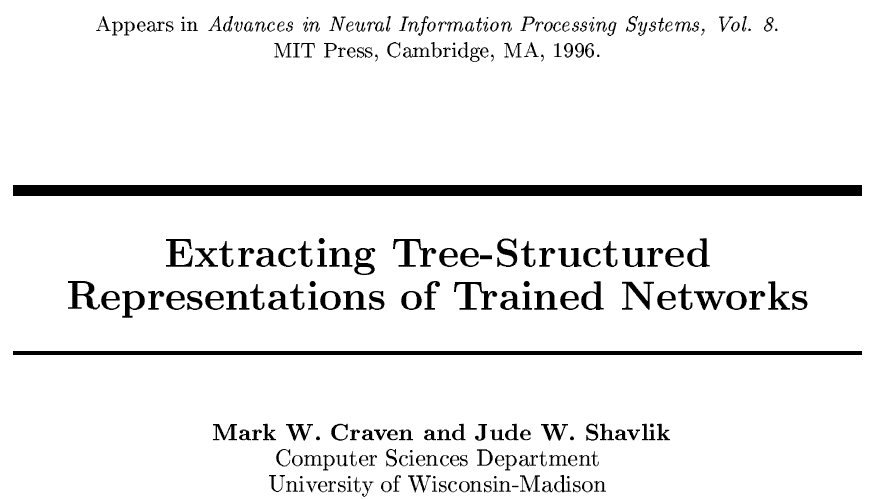
\includegraphics[width=6cm]{trepan-title.png}
\end{frame}

%%% FRAMEBREAK %%%

\begin{frame}{a frame}
with text
\end{frame}

\end{document}